% !TeX root = proceedings.tex
% 5쪽 프로시딩의 편집 본문. proceedings.tex에서 이 파일을 포함합니다.
\section{서론}
4족 보행 로봇은 시설 점검과 탐사처럼 다양한 지형을 이동하는 작업에 활용된다. 강화학습과 병렬 시뮬레이션으로 이러한 환경의 보행 정책을 학습할 수 있다\cite{ref1}. 다만 정상 상태에서 익힌 제어가 구동기 고장 이후에도 유효한지는 별도의 문제이다. 관절 토크가 저하되면 넘어지지 않더라도 명령한 속도와 방향을 유지하지 못할 수 있다. 따라서 고장 대응은 균형 유지와 명령 수행을 함께 평가해야 한다.

본 연구는 단일 관절 토크 저하 이후에도 보행과 속도 추종을 이어가도록 기존 교사·학생 공동학습을 적용한다\cite{ref4}. 교사는 시뮬레이션의 물리 조건을 사용하고, 학생은 최근 몸체·관절 반응으로 그 특징을 추정한다. 교사 특징을 학생 특징으로 점진적으로 대체하면서 제어 정책도 함께 갱신하며, 평가에서는 고장 위치와 손실률을 직접 입력받지 않는 학생 경로만 사용한다. Unitree A1의 12개 관절과 6개 손실률에서 정상 상태만 학습한 정책과 비교한다. 생존율과 속도 오차, 전방 이동량 및 명령 추종 시간율을 평가하여, 보행 유지가 명령 수행으로 이어지는지 확인하고 관절별 취약 조건을 분석한다.

\section{시스템 모델}

\subsection{시뮬레이션 환경 및 제어 구조}
Isaac Gym의 graphics processing unit (GPU) PhysX에서 Unitree A1을 모사한다\cite{ref2}. 각 다리는 hip, thigh, calf로 구성되며, 전체 관절은 12개이다. 정책의 목표 관절각을 proportional-derivative (PD) 제어기가 토크로 변환하고, 몸체·관절 반응을 다음 관측에 반영하여 제어를 반복한다\cite{ref1}. 로봇과 지형은 그림~\ref{fig:environment}, 제어 설정은 표~\ref{tab:system}과 같다. 행동 $a_t$는 기준 자세 $q^0$에 더할 관절각을 정한다. 0.02~s마다 새 목표를 출력하고, 그 사이에는 목표를 유지한 채 0.005~s 간격으로 물리를 계산한다.

\begin{figure}[!t]
\centering
\begin{minipage}[b]{.48\columnwidth}
\centering
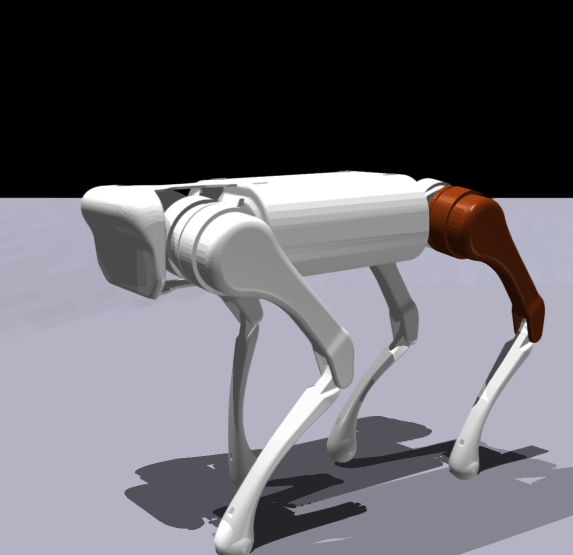
\includegraphics[width=\linewidth,trim=9bp 0bp 9bp 0bp,clip]{a1_robot_20261011_212425_original.png}\par
\small (a) Unitree A1
\end{minipage}\hfill
\begin{minipage}[b]{.48\columnwidth}
\centering
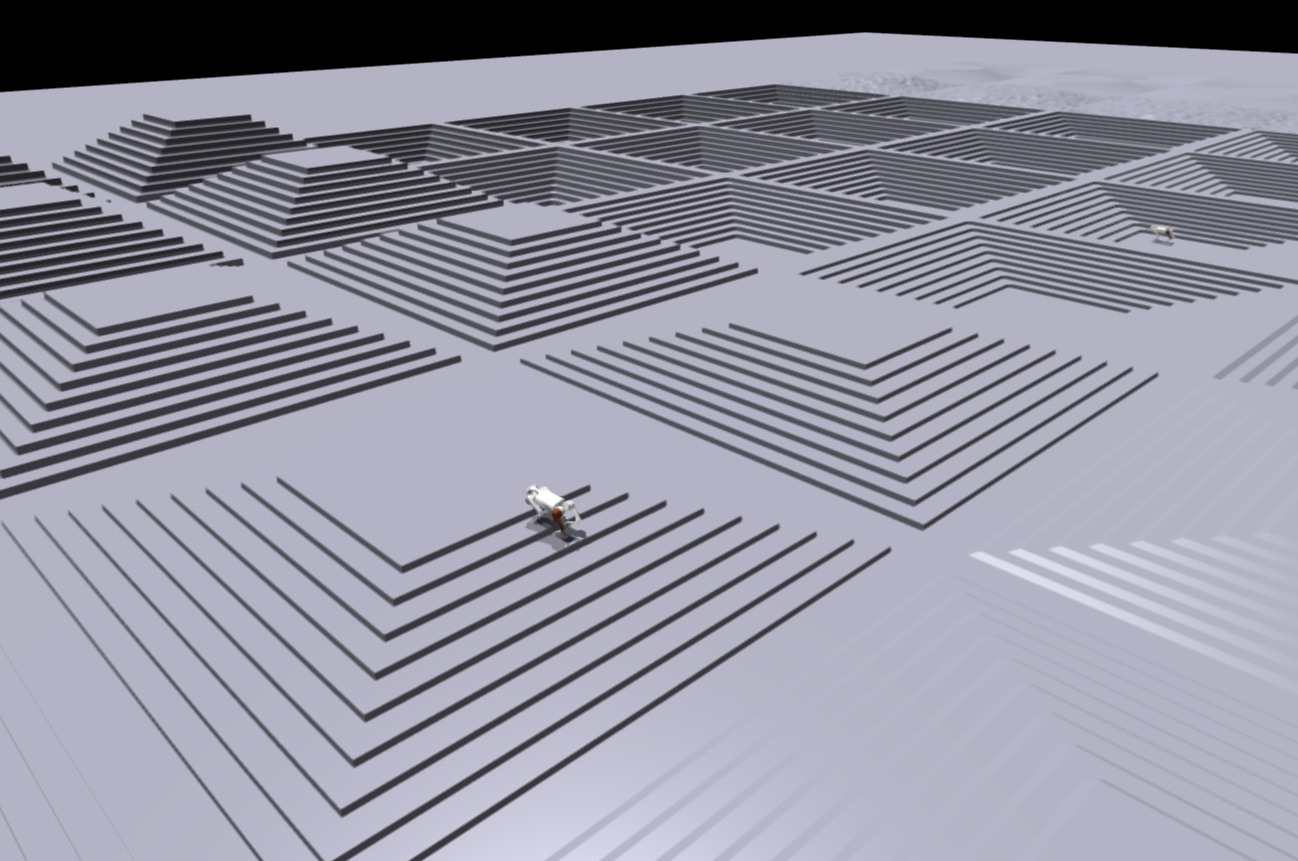
\includegraphics[width=\linewidth,trim=235 11 303 90,clip]{isaac_gym_original.png}\par
\small (b) Isaac Gym 지형
\end{minipage}
\caption{로봇 모델과 시뮬레이션 환경}
\label{fig:environment}
\end{figure}

\begin{table}[!t]
\caption{로봇 및 제어 설정}\label{tab:system}
\centering\paperTableFont
\begin{tabularx}{\columnwidth}{@{}lY@{}}
\toprule
Parameter & Value \\
\midrule
Actuated joints & 12 (hip, thigh, calf per leg) \\
Physics / policy interval & 0.005~s / 0.02~s \\
Joint target & $q^{des}=q^0+0.25a_t$ (rad) \\
Nominal PD gains & $K_p=20$~N$\cdot$m/rad; $K_d=0.5$~N$\cdot$m$\cdot$s/rad \\
\bottomrule
\end{tabularx}
\end{table}


\subsection{단일 관절 토크 저하 모델}
관절 토크 저하는 요구 토크의 일부만 출력되는 것으로 모델링한다\cite{ref6}. 손실률 $d\in[0,1]$에 대해 출력 배율은 $1-d$이며, $d=0.4$는 명목 출력의 40\% 손실을 뜻한다. PD 토크에 모터 강도 $m_j$와 고장 배율 $\eta_j$를 곱한 뒤 관절 한계 토크로 제한한다.
\begin{paperdisplay}[-0.83bp]
\begin{align}
\tau_j^{PD}&=K_p(q_j^{des}-q_j)-K_d\dot q_j,\label{eq:pd} \\
\tau_j&=\mathrm{clip}(m_j\eta_j\tau_j^{PD},-\tau_j^{max},\tau_j^{max}).\label{eq:torque}
\end{align}
\end{paperdisplay}
식~\eqref{eq:pd}, \eqref{eq:torque}에서 $q_j^{des}$, $q_j$, $\dot q_j$는 목표 관절각, 현재 관절각, 관절속도이며, $K_p$, $K_d$는 PD 이득이다. $\tau_j^{max}$는 관절 $j$의 최대 허용 토크이며, $\mathrm{clip}$은 출력을 $\pm\tau_j^{max}$로 제한한다. $m_j$는 [0.9, 1.1]에서 무작위화하여 고장과 별개인 $\pm10$\% 편차를 반영한다. 완전 손실($d=1$)에서는 능동 토크가 0이지만, 관절 잠금과 달리 수동 운동은 유지된다.

고장은 선택된 관절 $j_f$에서 시점 $t_f$에 발생하며, 나머지 관절의 배율은 1로 유지한다.
\begin{paperdisplay}[-0.17bp]
\begin{equation}
\eta_j(t)=
\begin{cases}
1-d, & j=j_f,\ t\geq t_f,\\
1, & \text{그 외},
\end{cases}.\label{eq:fault}
\end{equation}
\end{paperdisplay}
식~\eqref{eq:fault}의 $j_f$, $t_f$는 고장 관절과 발생 시점이다. 에피소드마다 관절 하나와 0, 20, 40, 60, 80, 100\% 중 하나의 손실률을 무작위로 선택한다. 시작 후 2~s부터 10~s 사이에 고장을 발생시키고 배율을 유지한다. 고장 전후를 한 에피소드에 포함하여, 정상 보행 중 반응이 달라져도 제어를 이어가도록 학습한다.


\section{교사·학생 공동학습 기반 보행 정책}

\subsection{관측 및 이력 표현}
고장 정보를 직접 받지 않는 학생에게는 행동 이후의 운동 반응이 단서가 된다. 따라서 현재 관측과 최근 1~s의 관측 이력을 함께 사용한다. 현재 관측 $o_t$는 로봇·명령 정보 $\tilde o_t$ 48차원과 지형 높이 187차원이다\cite{ref1}. $\tilde o_t$에는 선속도·각속도·중력 방향·속도 명령 각 3차원과 관절각 편차·관절속도·이전 행동 각 12차원이 포함된다. 각 관측의 기호·단위·차원은 표~\ref{tab:observation}과 같다.

\begin{table}[!t]
\caption{현재 관측의 구성}\label{tab:observation}
\centering\paperTableFont
\setlength{\tabcolsep}{3bp}
\begin{tabularx}{\columnwidth}{@{}Yccr@{}}
\toprule
Component & Symbol & Unit & Dim. \\
\midrule
Body linear velocity & $v_t$ & m/s & 3 \\
Body angular velocity & $\omega_t$ & rad/s & 3 \\
Projected gravity & $g_t$ & -- & 3 \\
Linear velocity command & $v_{xy}^{cmd}$ & m/s & 2 \\
Yaw-rate command & $\omega_z^{cmd}$ & rad/s & 1 \\
Relative joint position & $q_t-q^0$ & rad & 12 \\
Joint velocity & $\dot q_t$ & rad/s & 12 \\
Previous action & $a_{t-1}$ & -- & 12 \\
\midrule
Robot/command observation & $\tilde o_t$ & mixed & 48 \\
Terrain heights & $h_t$ & m & 187 \\
\midrule
Current observation & $o_t$ & mixed & 235 \\
\bottomrule
\end{tabularx}
\end{table}
교사는 마찰계수 1, 질량 1, 유효 모터 강도 12, PD 이득 24, 몸체 속도 6, 고장 표지 1의 총 45차원을 8차원 특징 $z_t^T$로 압축한다. 유효 모터 강도에는 손상 위치와 정도가 반영된다. 학생은 $H_t=[\tilde o_{t-49},\ldots,\tilde o_t]$의 $50\times48$ 이력을 convolutional neural network (CNN) 인코더로 처리하여 특징 $z_t^S$를 만든다\cite{ref4,ref3}. 부족한 과거 표본은 0으로 채운다. 현재 관측 235차원과 학생 특징 8차원을 결합하여 12차원 행동을 출력한다. 교사·학생 인코더와 정책의 차원 관계는 표~\ref{tab:encoders}에 정리하였다. 지형 높이는 이력에서 제외한다. 몸체 속도와 지형 높이는 시뮬레이터에서 얻으므로, 실제 로봇 적용에는 별도의 측정·추정이 필요하다.

\begin{table}[!t]
\caption{교사·학생 인코더와 정책의 입출력}\label{tab:encoders}
\centering\paperTableFont
\begin{tabularx}{\columnwidth}{@{}>{\raggedright\arraybackslash}p{28mm}Y@{}}
\toprule
Path & Input $\rightarrow$ output \\
\midrule
Teacher encoder & $45\rightarrow z_t^T\in\mathbb R^8$ \\
Student encoder & $H_t$: $50\times48\rightarrow z_t^S\in\mathbb R^8$ \\
Observation $o_t$ & $48+187=235$ \\
Training feature & $(1-\alpha)z_t^T+\alpha z_t^S$: 8 \\
Actor/Critic (train) & $[o_t,z_t]$: $235+8=243$ \\
Actor (inference) & $[o_t,z_t^S]$: $235+8=243\rightarrow a_t\in\mathbb R^{12}$ \\
\bottomrule
\end{tabularx}
\end{table}

\subsection{교사·학생 공동학습}
교사의 물리 정보는 학생의 평가 입력에 없다. 이에 교사 특징을 관측 이력으로 추정하는 구조와 특징 혼합 공동학습을 적용한다\cite{ref3,ref4}. 모방 오차가 남아 있어도 제어 정책이 학생 특징에 적응하도록, 다음 특징을 행동 정책(Actor)과 가치 함수(Critic)에 입력한다.

\begin{paperdisplay}[0bp]
\begin{equation}
z_t=(1-\alpha)z_t^T+\alpha z_t^S.\label{eq:latent}
\end{equation}
\end{paperdisplay}
식~\eqref{eq:latent}의 $\alpha$는 학생 특징의 혼합 비중이다. 사전학습 교사로 초기화한 뒤 공동학습 갱신 횟수 $n$에 따라 $\alpha(n)=\min(n/10000,1)$로 학생 비중을 높인다. 10,000회 이후에는 학생 특징만 사용하여 평가와 입력 경로를 맞춘다. 전환 중에는 proximal policy optimization (PPO) 손실에 모방항을 추가한다\cite{ref5}.

\begin{paperdisplay}[0.165bp]
\begin{equation}
\paperLoss=\paperLoss_{PPO}+\frac{1-\alpha}{B}\sum_{i=1}^{B}\|z_i^S-\mathrm{sg}(z_i^T)\|_2.\label{eq:loss}
\end{equation}
\end{paperdisplay}
스케줄과 손실은 선행 연구를 따른다\cite{ref4}. 식~\eqref{eq:loss}에서 $\paperLoss_{PPO}$는 정책·가치 학습 손실, $B$는 미니배치 크기, $i$는 배치 내 표본 번호, $\mathrm{sg}$는 모방 목표의 gradient 차단 연산이다. 교사는 전환 중에도 PPO로 갱신되며, $\alpha=1$ 이후에는 학생·Actor\allowbreak·\allowbreak{}Critic만 학습한다. 두 경로에서 학생 경로로 전환하는 구조는 그림~\ref{fig:architecture}과 같다.

\begin{figure}[!t]
\centering
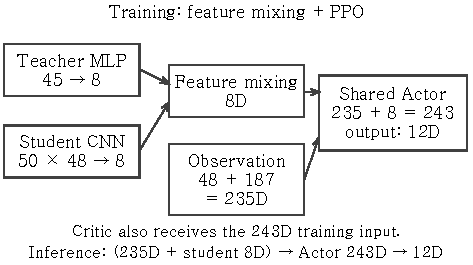
\includegraphics[width=\columnwidth]{paper_workflow_v8.pdf}
\caption{교사·학생 공동학습과 평가 시 학생 경로}\label{fig:architecture}
\end{figure}

\subsection{속도 추종 보상}
보상은 속도 추종과 안정적인 운동을 함께 유도한다\cite{ref1}. 평면 선속도와 yaw-rate(수직축 회전속도)의 추종항은 오차가 작을수록 큰 값을 갖는다.

\begin{paperdisplay}[-0.335bp]
\begin{align}
r_v&=\exp\left(-\|v_{xy}-v_{xy}^{cmd}\|_2^2/0.25\right),\label{eq:rv}\\
r_\omega&=\exp\left(-(\omega_z-\omega_z^{cmd})^2/0.25\right).\label{eq:rw}
\end{align}
\end{paperdisplay}
식~\eqref{eq:rv}, \eqref{eq:rw}에서 $v_{xy}$와 $\omega_z$는 평면 선속도와 수직축 각속도이며, 위첨자 $cmd$는 명령값이다. 두 식의 0.25는 오차에 따른 보상 감소 폭을 정하는 계수이다. 표~\ref{tab:reward}의 비용항은 수직·roll/pitch 운동과 과도한 토크, 급격한 행동 변화 등을 억제한다. 원시 물리량으로 계산한 가중합에 제어 간격을 곱하고 음수 총보상은 0으로 제한한다. PPO로 할인 보상합을 최대화한다.


\begin{table}[!t]
\caption{제어 간격 적용 전 보상항별 가중치}\label{tab:reward}
\centering\paperTableFont
\begin{tabularx}{\columnwidth}{@{}Yl@{}}
\toprule
Reward term & Weight \\
\midrule
Planar velocity tracking / yaw-rate tracking & 1 / 0.5 \\
Squared vertical velocity & $-2$ \\
Squared roll/pitch angular velocity & $-0.05$ \\
Squared joint torque & $-2\times10^{-4}$ \\
Squared joint acceleration & $-2.5\times10^{-7}$ \\
Squared action change & $-0.01$ \\
Disallowed contact count & $-1$ \\
Joint-limit excess & $-10$ \\
Foot air-time reward & 1 \\
\bottomrule
\end{tabularx}
\end{table}

\subsection{정책 학습 환경 및 설정}
물리 조건에 따라 달라지는 고장 후 반응을 학습하도록 마찰계수 0.5에서 1.25, 추가 질량 0에서 2~kg, 명목 모터 강도 $\pm10$\%를 무작위화하였다. PD 이득도 $K_p$ $\pm5$\%, $K_d$ $\pm10$\%로 변화시키고 혼합 지형과 주기적인 외란을 적용하였다.

교사 인코더는 multi-layer perceptron (MLP)으로, 은닉층 [512, 256, 128]과 exponential linear unit (ELU)를 사용한다\cite{ref4}. 본 구현의 Actor·Critic도 같은 은닉층 크기를 갖는다. 학생 인코더는 rapid motor adaptation (RMA) 계열로, 48차원 프레임을 64차원으로 변환한 뒤 세 개의 1차원 합성곱 층을 거쳐 8차원 특징을 출력한다\cite{ref3}. Actor·Critic 입력은 현재 관측과 혼합 특징의 243차원이다.
% Provenance: Saving the Limping v3, IV-A (teacher MLP and 50-frame CNN).
% RMA, IV Implementation Details (three temporal Conv1d layers).
% Local implementation: legged_gym/learning/joint_teacher_student_actor_critic.py;
% selected JT configuration uses student_embedding_dim=64 (RMA paper uses 32).
% Actor/critic [512,256,128] are our implementation choices; STL actor is [256,128].

병렬 환경 4,096개에서 환경당 24개 제어 시점의 경험으로 PPO를 갱신한다. 미래 보상의 가중치를 정하는 할인 계수(discount factor) $\gamma=0.99$, generalized advantage estimation (GAE) 계수 0.95, clip 계수 0.2, 갱신당 5회 학습과 4개 미니배치를 사용한다. 공동학습 초기 학습률(learning rate)은 $10^{-5}$이고 Kullback-Leibler (KL) divergence에 따라 조절한다. 학습 과정은 그림~\ref{fig:learning}, 토크 손실률별 성능은 그림~\ref{fig:performance}에 제시한다.


\section{시뮬레이션 결과 및 평가}

\subsection{평가 조건과 지표}
정상 상태만 학습한 정상학습 정책(Normal)과 고장 조건에서 공동학습한 고장대응 정책(Student)을 비교한다. Normal은 현재 관측만, Student는 현재 관측과 이력 특징을 사용한다. 고장 학습과 이력 표현이 함께 적용된 정책의 비교이며, 초기 물리 조건·지형·고장 일정은 동일하게 맞춘다.

관절·손실률 조합마다 평가 시드 3개와 시드별 16회 시행을 배정한다. 조건당 48회, 손실률당 576회, 정책당 3,456회이다. 고장 후 20~s를 관찰하며 종료된 로봇은 다시 시작하지 않는다. 손실률 0\%도 같은 구간으로 집계한다. 각 정책은 학습 시드 1에서 한 번 학습하여, 학습 초기화에 따른 변동성은 평가 범위에 포함하지 않았다.

\begin{table}[!t]
\caption{정책 비교를 위한 평가 조건}\label{tab:evaluation}
\centering\paperTableFont
\begin{tabularx}{\columnwidth}{@{}lY@{}}
\toprule
Item & Setting \\
\midrule
Command & $v_x$=0.5~m/s; $v_y$=$\omega_z$=0 \\
Conditions & 12 joints $\times$ $d\in\{0,0.2,0.4,0.6,0.8,1\}$ \\
Onset / observation & 2–10~s / 20~s after onset \\
Trials & Evaluation seeds 301–303 $\times$ 16; 48 per joint/loss \\
Failure & Base contact force $> 1$~N; pre-fault failure included \\
\bottomrule
\end{tabularx}
\end{table}

\begin{figure}[!t]
\centering
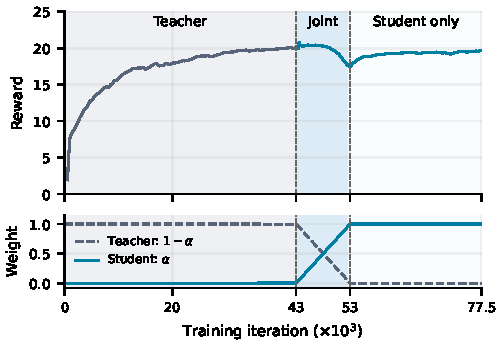
\includegraphics[width=\columnwidth]{paper_learning_v10.pdf}
\caption{학습 단계별 평균 에피소드 보상(상단, 500회 이동평균)과 교사·학생 특징의 혼합 비중(하단)}\label{fig:learning}
\end{figure}
표~\ref{tab:evaluation}과 같이 평가하며, 혼합 지형과 물리 무작위화는 유지하고 관측 잡음·외부 밀기·curriculum은 해제한다. 생존율은 고장 전 실패를 포함한 전체 시행 중 관찰 종료까지 생존한 비율이다. 추종 오차는 고장 후 생존 구간의 표본 $K$개에 대한 root mean square error (RMSE)로 계산한다.

\begin{paperdisplay}[-0.17bp]
\begin{equation}
\mathrm{RMSE}_u=\sqrt{\frac{1}{K}\sum_{k=1}^{K}(u_k-u^{cmd})^2}.\label{eq:rmse}
\end{equation}
\end{paperdisplay}
\begingroup\widowpenalty=10000
식~\eqref{eq:rmse}의 $u_k$는 표본 $k$의 속도이며, 명령은 $u\in\{v_x,v_y,\omega_z\}$에 대해 각각 0.5~m/s, 0~m/s, 0~rad/s이다. RMSE에서 빠지는 낙상 이후 시간까지 반영하도록, 전체 관찰 시간 중 생존하며 세 축의 허용오차를 만족한 비율 $Q_{20}$을 함께 사용한다.
\par\endgroup
\begin{paperdisplay}[-0.665bp]
\begin{align}
Q_{20}&=\frac{100}{NT}\sum_{i=1}^{N}\int_0^T
 A_i(t)\,C_i(t)\,dt,\label{eq:q20}\\
C_i(t)&=\paperIndicator\!\left\{
\begin{aligned}
|v_{x,i}(t)-0.5|&\leq0.1,\\
|v_{y,i}(t)|&\leq0.1,\\
|\omega_{z,i}(t)|&\leq0.2
\end{aligned}\right\}.\label{eq:tracking}
\end{align}
\end{paperdisplay}
식~\eqref{eq:q20}, \eqref{eq:tracking}에서 $C_i(t)$는 세 축 오차가 모두 허용 범위에 들면 1, 그 외에는 0인 지시함수이다. $t$는 고장 후 시간, $T=20$~s, $N$은 시행 수이며 $A_i(t)$는 생존 시 1, 종료 후 0이다. 허용오차 단위는 m/s와 rad/s이다. 낙상 이후도 분모에 남겨 미추종으로 처리하며, 엄격 추종률 $Q_{10}$은 허용오차를 절반으로 줄인다.

\begin{figure}[!t]
\centering
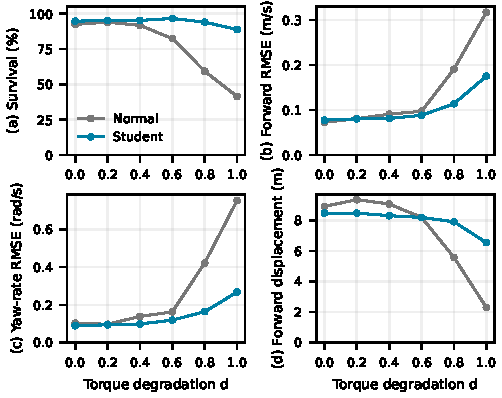
\includegraphics[width=\columnwidth]{paper_metrics_v10.pdf}
\caption{토크 손실률에 따른 생존율, 전진속도·yaw-rate 추종 오차 및 전방 순변위}\label{fig:performance}
\end{figure}

전방 순변위 $D_\parallel$는 고장 순간부터 마지막 생존 표본까지의 세계좌표 xy 변위를 고장 순간의 수평 전방 $\hat u^f$에 \mbox{투영한 값이다.}
\begin{paperdisplay}[-0.165bp]
\begin{equation}
D_{\parallel}=(x^{last}-x^f)^\top\hat u^f.\label{eq:displacement}
\end{equation}
\end{paperdisplay}
식~\eqref{eq:displacement}의 $x^f$, $x^{last}$는 고장 순간과 마지막 생존 표본의 세계좌표 xy 위치이다. 고장 전 종료된 시행은 0으로 처리한다. 몸체 좌표계 속도 적분과 달리 고장 당시의 \mbox{전방으로} 이동한 정도를 나타낸다. 명령대로 0.5~m/s로 20~s 동안 직진한 기준 이동거리는 10~m이다.


\subsection{학습 과정}
그림~\ref{fig:learning}에서 학생 특징으로 전환할 때 감소한 보상은 후속 학습에서 회복된다. 교사를 43,000회까지 학습한 뒤 53,000회까지 $\alpha$를 0에서 1로 높였고, 77,500회의 학생 정책을 평가하였다. 전환 완료 시점의 평균 보상은 17.52에서 최종 19.70으로 증가하였다. 이는 바뀐 입력으로 정책이 보행을 학습한 과정이며, 고장 대응 성능은 다음 절의 조건별 평가로 확인한다.


\subsection{토크 저하에 따른 생존 및 명령 추종 성능}
그림~\ref{fig:performance}에서 정책 간 차이는 토크 손실률이 커질수록 뚜렷해진다. 완전 손실의 생존율은 Normal 41.49\%에서 Student 88.89\%로 높아지고, 전진속도·yaw-rate RMSE는 각각 0.317에서 0.175~m/s, 0.753에서 0.268~rad/s로 감소한다. 보행 유지와 생존 구간의 속도 추종이 함께 개선된 것이다. 표~\ref{tab:performance_gain}에서 낮은 손실률의 차이는 작고, 0에서 40\%의 전방 순변위는 Student가 오히려 작다. 반면 80\% 이상에서는 생존율과 이동량의 차이가 함께 커진다. 따라서 이점은 모든 조건에 고르게 나타나기보다 강한 토크 저하에 집중된다. 완전 손실의 전방 순변위도 2.31~m에서 6.56~m로 증가하지만 기준 10~m에는 미치지 못한다. 생존율 향상이 정상 이동 성능의 회복을 뜻하지는 않으며, 저하된 구동 능력에서 이동을 부분적으로 유지한 결과이다. 추종 시간율은 이 차이를 더 직접적으로 보여준다. 정상 조건의 $Q_{20}$은 두 정책 모두 약 80\%지만, 완전 손실에서는 16.57\%에서 41.07\%로 증가한다. Student도 20~s 중 평균 8.21~s만 세 축의 허용오차를 만족한다. 엄격한 $Q_{10}$은 4.43\%에서 12.30\%로 개선되나, 높은 생존율에 비해 정밀 추종의 개선 여지는 크다.

\begin{table}[!t]
\caption{정책별 성능 차이(Student−Normal)}\label{tab:performance_gain}
\centering\paperTableFont
\setlength{\tabcolsep}{2pt}
\begin{tabularx}{\columnwidth}{@{}>{\centering\arraybackslash}p{8mm}*{4}{>{\centering\arraybackslash}X}@{}}
\toprule
Loss\newline (\%) & Survival\newline (\%p) & $v_x$ RMSE\newline (m/s) & yaw RMSE\newline (rad/s) & Forward\newline disp. (m) \\
\midrule
0 & +2.26 & +0.0047 & -0.0133 & -0.437 \\
20 & +1.22 & -0.0003 & -0.0027 & -0.881 \\
40 & +3.47 & -0.0094 & -0.0399 & -0.766 \\
60 & +14.24 & -0.0090 & -0.0437 & -0.004 \\
80 & +34.72 & -0.0767 & -0.2578 & +2.333 \\
100 & +47.40 & -0.1418 & -0.4850 & +4.250 \\
\bottomrule
\end{tabularx}
\end{table}

\subsection{관절별 고장 대응 성능}
\begin{figure}[!t]
\centering
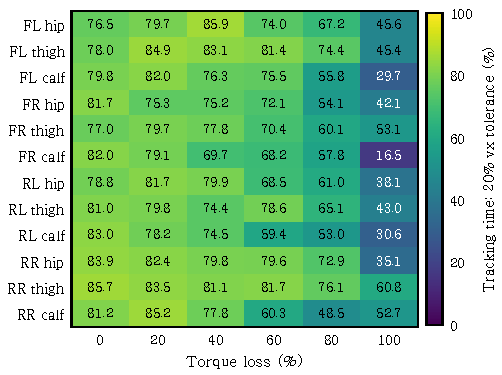
\includegraphics[width=\columnwidth]{paper_joint_tracking20_v12.pdf}
\caption{관절 및 토크 손실률별 Student 명령 추종 시간율 $Q_{20}$(\%)}\label{fig:joint_tracking}
\end{figure}
관절별 결과는 평균 성능에 가려진 취약 조건을 보여준다. 그림~\ref{fig:joint_tracking}는 Student의 $Q_{20}$을 같은 0에서 100\% 색 범위로 비교한다. front left (FL)/front right (FR)은 좌/우 앞다리, rear left (RL)/rear right (RR)은 좌/우 뒷다리이다. 완전 손실에서 RR thigh는 60.84\%, FR calf는 16.49\%이다. FR calf는 생존율이 83.33\%임에도 추종 시간이 짧아, 균형 유지 이후의 명령 수행이 과제로 남는다. 손실률 60\% 이상에서 네 calf의 평균 추종 시간율은 hip·thigh보다 낮아, calf 토크 저하에서 취약해지는 경향이 있다. 다만 완전 손실의 RR calf는 RR hip보다 높아 위치별 예외도 나타난다. 관절 종류별 보완이 필요하지만, 이 결과만으로 취약성의 원인을 특정할 수는 없다.

\section{결론 및 향후 연구}
기존 교사·학생 공동학습을 단일 관절 토크 저하에 적용하여, 정상학습 정책보다 강한 저하에서 생존·속도 추종·전방 이동이 개선됨을 확인하였다. 그러나 높은 생존율에도 추종 시간은 제한적이며, calf 고장에서 취약성이 남았다. 따라서 낙상 여부와 명령 수행을 함께 평가할 필요가 있다. 결과는 시뮬레이션의 단일 관절 저하와 전진 명령에 한정된다. 향후 다양한 명령과 학습 시드에서 검증하고, 다중 관절 저하와 관절 잠금으로 확장할 예정이다.

\begin{thebibliography}{9}
\paperreferencefont
% 좁은 단에서 영문 참고문헌의 단어 간격이 벌어지지 않도록 왼쪽 정렬한다.
\ifproceedings\else\raggedright\fi
\bibitem{ref1} N. Rudin, D. Hoeller, P. Reist, and M. Hutter, ``Learning to walk in minutes using massively parallel deep reinforcement learning,'' in Proc. 5th Conf. Robot Learning (CoRL), London, UK, PMLR, vol. 164, pp. 91-100, 2022.
\bibitem{ref4} D. Liu, T. Zhang, J. Yin, and S. See, ``Saving the limping: Fault-tolerant quadruped locomotion via reinforcement learning,'' arXiv preprint arXiv:2210.00474v3, 2023.
\bibitem{ref2} V. Makoviychuk et al., ``Isaac Gym: High performance GPU based physics simulation for robot learning,'' in Proc. Neural Information Processing Systems Track on Datasets and Benchmarks (NeurIPS), Virtual, vol. 1, 2021.
\bibitem{ref6} X. Wu, W. Dong, H. Lai, Y. Yu, and Y. Wen, ``Adaptive control strategy for quadruped robots in actuator degradation scenarios,'' in Proc. 5th Int. Conf. Distributed Artificial Intelligence (DAI), Singapore, pp. 1-13, 2023.
\bibitem{ref3} A. Kumar, Z. Fu, D. Pathak, and J. Malik, ``RMA: Rapid motor adaptation for legged robots,'' in Proc. Robotics: Science and Systems (RSS), Virtual, 2021.
\bibitem{ref5} J. Schulman, F. Wolski, P. Dhariwal, A. Radford, and O. Klimov, ``Proximal policy optimization algorithms,'' arXiv preprint arXiv:1707.06347, 2017.
\end{thebibliography}
